%%%%%%%%%%%%%%%%%%%%%%%%%%%%%%%%%%%%%%%%%
% MPhys Report
% Semester 2
% 
% Started on 04/05/16
% Author: Rhiannon Jones
% 4th Year MPhys Sem2
% 
%%%%%%%%%%%%%%%%%%%%%%%%%%%%%%%%%%%%%%%%%

%----------------------------------------------------------------------------------------
%	PACKAGES AND OTHER DOCUMENT CONFIGURATIONS
% Downloads the required packages for certain features
%----------------------------------------------------------------------------------------

\documentclass[11pt]{article}
\usepackage[utf8]{inputenc}
\usepackage{amsmath}
%\usepackage{amsfonts}
\usepackage[sc]{mathpazo}
\linespread{1.05}         % Palladio needs more leading (space between lines)
\usepackage[T1]{fontenc}
%\renewcommand*\rmdefault{Type1}
\usepackage{ulem}
\usepackage{amssymb}
\usepackage{verbatim}
\usepackage{graphicx}
\usepackage{courier}
\usepackage{cite}
\linespread{1.2} % Line spacing - Palatino needs more space between lines
% Load all packages needed for all sub−files:
\usepackage{xcolor}
\definecolor{purpleX}{rgb}{0.573,0,1}
\definecolor{greenX}{rgb}{0.349,0.831,0.329}
\usepackage{geometry}
 \geometry{
 a4paper,
 total={210mm,297mm},
 left=28mm,
 right=28mm,
 top=30mm,
 bottom=30mm,
 }% Document margins
\usepackage{multicol} % Used for the two-column layout of the document
\usepackage{color}
\setlength{\columnseprule}{1pt}
\def\columnseprulecolor{\color{gray}}
\usepackage[hang, small,labelfont=bf,up,textfont=it,up]{caption} % Custom captions under/above floats in tables or figures
\usepackage{booktabs} % Horizontal rules in tables
\usepackage{float} % Required for tables and figures in the multi-column environment - they need to be placed in specific locations with the [H] (e.g. \begin{table}[H])
\usepackage{paralist} % Used for the compactitem environment which makes bullet points with less space between them
\usepackage{abstract} % Allows abstract customization
\renewcommand{\abstractnamefont}{\LARGE} % Set the "Abstract" text to bold
\renewcommand{\abstracttextfont}{\itshape} % Set the abstract itself to italic text
\usepackage{titlesec} % Allows customization of titles
\titleformat{\section}[block]{\large}{\thesection.}{.8em}{} % Change the look of the section titles
\titleformat{\subsection}[block]{\scshape\itshape}{\thesubsection.}{.8em}{} % Change the look of the section titles

%----------------------------------------------------------------------------------------
%	TITLE SECTION
%----------------------------------------------------------------------------------------

\title{\vspace{5mm}\fontsize{20pt}{12pt}\selectfont A preliminary investigation into determining \\ \vspace{3mm} CC0\(\pi\) cross-section sensitivities in SBND \\ } % Article title

\author{
    \date{}
}

%----------------------------------------------------------------------------------------

\begin{document}

\nocite{*}

\pagenumbering{gobble}

\maketitle % Insert title

\vspace{-9mm}

\begin{figure}[h!]
    \center
    \includegraphics[scale=0.6]{images/UoL_CoA.pdf}
\end{figure}

\vspace{3mm}

\begin{center}

    \large Rhiannon Jones\\
    \normalsize University of Liverpool \\
    \normalsize School of Physical Sciences \\ % Institution
    \normalsize rjones@hep.ph.liv.ac.uk \\ 
    \vspace{3mm}
    \normalsize 1\( ^{ \mbox{\footnotesize st } } \) year PhD report \\

\end{center}

\vspace{6mm}
%----------------------------------------------------------------------------------------
%	ABSTRACT
%----------------------------------------------------------------------------------------
\begin{abstract}
    Random stuff
\end{abstract}
\newpage
%----------------------------------------------------------------------------------------
%	ARTICLE CONTENTS
%----------------------------------------------------------------------------------------
\pagenumbering{arabic}
\section{Introduction}
\label{sec:intro}

Neutrino physics is at the core of current high energy research. One of the profound discoveries made in recent years was the observation of neutrino flavour oscillations by the Super-Kamiokande (Super-K) experiment, which was the first confiramtion that physics existed beyond the standard model of particle physics. In brief, neutrinos described by the standard model would be massless particles, but since the flavours are made up of superpositions of mass states, the oscillation of
the flavour states implies that the relative mass states are different, and therefore non-zero \cite{nuInt}.

    Future, long-baseline,  neutrino experiments such as the Deep Underground Neutrino Experiment (DUNE) and Hyper-Kamiokande (Hyper-K) are hoping to investigate some of the most fundamental questions we are still asking: Why does the universe constist of matter, and not anti-matter? What is the neutrino mass heirarchy? Neutrino research is an extremely active field. Optimising the current and future detectors to maximise the accuracy of all interaction anaylses is a crucial step towards obtaining concrete answers to these questions. 

    A brief introduction to the topics covered in this report is as follows, more detail on each will be given in later sections. 

\subsection{Neutrino interactions}

Due to the elusive nature of the neutrino, directly observing one in a detector isn't possible. It is therefore necessary to infer their existence from particles produced when they interact. Since this process relies upon the reconstruction capability of the experiment, purpose-built detectors will attempt to maximise the efficiency of this.

Another property of the neutrino which poses a significant difficulty within detectors is their interaction probability, or cross-section. A typical neutrino cross-section is on the order of $ 10^{-44} $ cm$^{2}$ which corresponds to $\sim$1 interaction every 10 light years in steel, for neutrinos with only a few MeV energy \cite{nuOsc}. This fact introduces the need for the interacting neutrinos to have high energies in these dedicated experiments, if we are to sufficiently reduce their mean free path. More detail on this topic will be discussed in section~\ref{sec:NIP}.

\subsection{Cross-sections}
   
    In order to correctly model neutrino events within a specific detector geometry and material, certain parameters have to be known. In particular, the probability of an interaction taking place - its cross-section - is required for each possible interaction the neutrino could undergo. Cross-section measurements are therefore a necessity for the generators, and consequently the future detector studies mentioned earlier. 
    
    The extent of our current knowledge of charged current neutrino cross sections is shown in Figure~\ref{fig:xsecCurr}. The plot contains cross-section information from multiple types of neutrino experiment, differing in both target material and detector machinery. A feature of this plot which is of the most interest to a Short Baseline Near Detector (SBND) cross-section study in particular is the lack of precision in the measurements made towards the lower energy region \cite{xsecCurr}. SBND will not only be operational at this energy range, but it will also have substantial enough statistics to potentially make a significant contribution to improving the current knowledge in this region.

    %CC cross-sections
    \begin{figure}[h!]
        \center
        \includegraphics[width=.8\textwidth]{images/current_cross_sec_knowledge.pdf}
        \put(-68, -15){\Large E$_{\nu}$ ( GeV )}
        \put(-375, 50){\Large \rotatebox{90}{$\sigma_{\nu}$ / $\Delta$E$_{\nu}$ ( 10$^{-38}$ cm$^{2}$ / GeV ) }}
        \caption{A compilation of the total cross-section data across the $\sim$1 MeV to $\sim$100 GeV energy range. Including a breakdown in terms of the quasi-elastic, QE, resonant, RES and deep inelastic scattering, DIS, topologies \cite{xsecCurr}. }
        \label{fig:xsecCurr}
    \end{figure}

    The scale of contribution SBND could make to this area of physics would in turn improve the predictions made by event generators for the next generation of neutrino experiments. Cross-sections will be discussed further in section~\ref{sec:XSec}.
    
\subsection{GENIE and the GENIE-Professor global fits}

GENIE is the world leading Monte Carlo neutrino interaction generator. Generators are a crucial machinery in all high energy physics analyses as they use theoretical models to produce predictions of how and where neutrino interactions will occur in specific detector geometries \cite{genie}. With this information, comparisons between experimental data and theoretical predictions can be drawn, the models can be updated and potential new physics can be explored.

    Generators such as GENIE bridge the gap between theory and experiment, whilst also providing opportunities to prepare simulations and perform sensitivity studies for the next generation of neutrino experiments.

    Alongside building state-of-the art detectors and making high precision cross-section measurements to improve current and future neutrino physics analyses, the predictions made by the generators can be improved by taking existing neutrino data and performing a fit of the models to them. 

    An effort to do this is currently being carried out by GENIE, using the Professor software framework, which was written with this purpose for experiments at the LHC \cite{prof}. The ultimate goal of this exercise is to perfom a global fit to all neutrino scattering data and consequently produce comprehensive model configurations to further optimise the predictions made for the next generation of neutrino experiments. This work will and GENIE's role in current and future neutrino experiments will be discussed further in section~\ref{sec:GF}.

\clearpage


%---------------------------------------------------------------------------------------------------------------
\section{Neutrino Interaction Phenomenology in the few-GeV Energy Range}
\label{sec:NIP}

\subsection{Dominant topologies}
\subsection{Golden channel}
\subsection{Signal}
\subsection{Potential backgrounds}
\subsection{\textbf{Maybe some results here?}}

\clearpage


%---------------------------------------------------------------------------------------------------------------
\section{Theory and Recent Measurements of CC0\( \pi \) Cross-Section}
\label{sec:XSec}

\subsection{Cross-sections}
Inc. equations
\subsection{Method}
\subsection{Unfolding}
\subsection{Results}
Plots and cross-section values

\clearpage


%---------------------------------------------------------------------------------------------------------------
\section{A Global Fit of CC0\( \pi \) Data}
\label{sec:GF}

%Plan

\subsection{GENIE and the comparisons}
GENIE applies theoretical physics models, composed of both physical and unphysical parameters, to detector geometries and materials to build experiment-specific neutrino interaction predictions \cite{genie}. The collaboration is in the process of improving configurations of these models for the purpose of optimising the accuracy of the predictions.

    An archive of experimental data is publicly available, and provides the key ingredient to this configuration update. Comparing the models with these data sets allows for a direct performance evaluation of the predictions, whilst fitting the models to the data enables the parameters to be tuned and consequently improve the prediction.

Summaries of the configuration of the GENIE models are as follows:

\begin{figure}[h!]
    \centering
    \includegraphics[width=\textwidth]{images/model_summaries.pdf}
    \caption{A brief overview the features which make up the individual model configurations in GENIE. These models will eventually all be tuned.}
    \label{tab:modelConfigs}
\end{figure}


Details on the first model to be tuned (G16\_01b) are as follows: 

\begin{itemize}
    \item Includes Empirical MEC
    \item CCQE process is Llewellyn-Smith Model
    \item Dipole Axial Form Factor - Depending on M\(_{A}\) = 0.99 GeV
    \item Nuclear model: Fermi Gas Model - Bodek, Ritchie
\end{itemize}

this model takes the updated default GENIE model (G16\_01a) and additionally addresses the abnormalities seen in recent experiments by incorporating the MEC interaction, described schematically in terms of the theoretical models involved in Figure~\ref{fig:MECSchem} \cite{MEC}. 

\begin{figure}[h!]
    \centering
    \includegraphics[width=.6\textwidth]{images/mec_model_genie.png}
    \caption{The models involved in the construction of the MEC model in neutrino event generation.}
    \label{fig:MECSchem}
\end{figure}

Datasets currently involved in the fit come from MiniBooNE, T2K and Minerva. An example of a comparison between the MiniBooNE \(\bar{\nu}_{\mu}\) CCQE data set from 2013 and 4 different GENIE predictions is shown in Figure~\ref{fig:MBComp}.

\begin{figure}[h!]
    \centering
    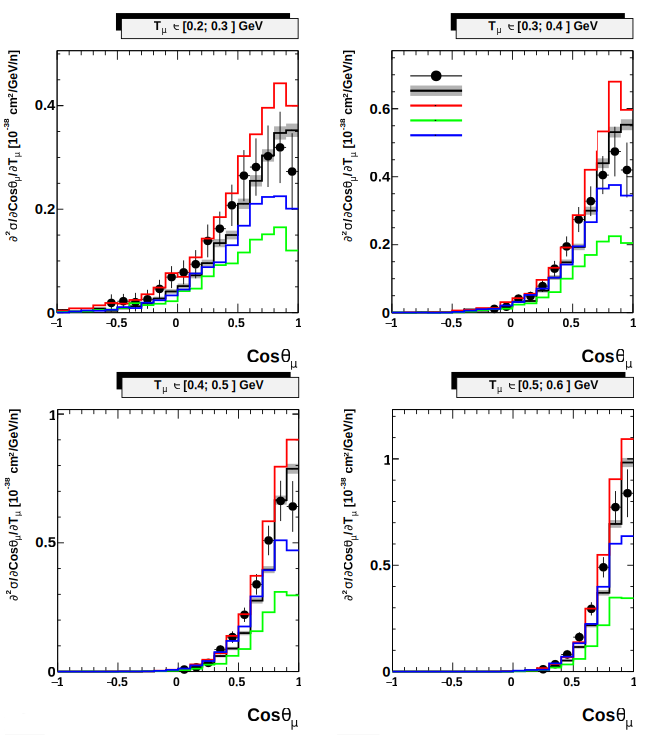
\includegraphics[width=\textwidth]{images/MB_Comp_numubar.pdf}
    \put(-120,450){\scriptsize MiniBooNE \(\bar{\nu}_{\mu}\)CCQE, 2013}
    \put(-120,440){\scriptsize G00\_00a}
    \put(-120,430){\scriptsize G00\_00b}
    \put(-120,420){\scriptsize G16\_01a}
    \put(-120,410){\scriptsize G16\_02b}
    \caption{An example comparison between 4 GENIE models (described briefly in Figure~\ref{tab:ModelConfigs}) and MiniBooNE \(\bar{\nu}_{\mu}\)CCQE data from 2013. The models fit the data with varying accuracies. It can be seen that even the closest fitting model is does not perfectly predict the trend seen in the data, therefore tuning is needed to fully optimise these fits.}
    \label{fig:MBComp}
\end{figure}

\begin{itemize}
    \item Tensions
\end{itemize}

\subsection{Professor}

\subsection{The fit}
\begin{itemize}
    \item Description of global fit
    \begin{itemize}
        \item How it works
        \item Schematic
    \end{itemize}
\end{itemize}

\subsection{Results}
\begin{itemize}
    \item Results 
\end{itemize}



\clearpage


%---------------------------------------------------------------------------------------------------------------
\section{Prospects for a CC0\( \pi \) Measurement at SBND and Sensitivity Esimates}
\label{sec:Prospects}

\subsection{SBND sensitivity}
\subsection{Future}

\clearpage


%---------------------------------------------------------------------------------------------------------------

\section{Discussion}

\input{discussion.tex}

\newpage

%----------------------------------------------------------------------------------------
%	REFERENCE LIST
%----------------------------------------------------------------------------------------
\bibliographystyle{unsrt}
\bibliography{bib}

    %\bibitem{nuOsc} The Super Kamiokande Collaboration. Evidence for oscillation of atmospheric neutrinos. arXiv:hep-ex/9807003v2 31 Aug 1998.

    %\bibitem{nuInt} K. McFarland. Neutrino Interactions. arXiv:0804.3899v1 [hep-ex] 24 Apr 2008.
%---------------------------------------------------------------------------------------
\end{document}
